\subsection{Binäres Culling}

Wir können beide Probleme der ersten Implementation
mit einer neuen Methode lösen.
Wir betrachten dabei eine Reihe von Voxels als einen
64-Bit Integer, wobei die einzelnen Bits darstellen,
ob sich dort ein Voxel befindet.
Es werden dabei 64 Bits gebraucht und nicht nur 32,
da man für das Culling auch wissen muss,
welche Voxels sich am Rand eines Chunks befinden,
und ein Chunk 32 Voxels lang ist.
Somit könnten die Voxels in einem Chunk
(und dem Rand) als ein 2 dimensionales
Array von 64-Bit Integers dargestellt werden,
wobei die 2 Dimensionen des Arrays die
$y$- und $z$-Achse darstellen und der Integer eine
Reihe von Voxels in der $x$-Achse darstellt.
Der Vorteil davon ist, dass wir somit in der
$x$-Achse binäre Arithmetik anwenden können für
das Culling, was sehr schnell ist.

Beim Culling müssen wir die Seiten von
Voxels finden, die nicht von einem anderen Voxel
verdeckt werden.
Mit binärer Arithmetik geht dies jetzt sehr einfach:

\begin{lstlisting}[language=Rust]
fn find_faces(mask: u64) -> u32 {
	((mask & !(mask >> 1)) >> 1) as u32
}
\end{lstlisting}
%
Diese Funktion gibt eine Bitmaske für alle Voxels,
die von links sichtbar sind.
Dabei ist das \code{mask \& !(mask >> 1)} zuständig,
die sichtbaren Seiten zu erkennen.
Definiert man also eine Funktion mit
\code{mask \& !(mask << 1)}, dann bekommt man alle,
die von rechts sichtbar sind.
Das \code{((..) >> 1) as u32} ist dann zuständig,
die einzelnen Bits, die den Rand des Chunks beschreiben,
zu entfernen, da diese nicht mehr gebraucht sind.
Diese neue Bitmaske kann dann wie folgt verwendet
werden, um die Seiten der Voxels zu kreieren:

\begin{lstlisting}[language=Rust]
let mut mask = /* Bitmaske von dieser Reihe von Voxels */;
let mut k = 0;
while mask != 0 {
	let zeros = mask.trailing_zeros();
	mask = (mask >> zeros) & !1;
	k += zeros;
	// berechne die position dieser Seite basierend auf k,
	// und erstelle dann ein Mesh dafuer...
}
\end{lstlisting}

Um diese Funktion anwenden zu können, müssen
wir die Bitmaske aber erst konstruieren.
Dies werden wir für jede Achse wiederholen,
da jede Bitmaske nur für eine Achse anwendbar ist:

\begin{lstlisting}[language=Rust]
for ([x,y,z], block) in chunk.blocks.iter_xyz() {
	if block_models[&block.id].should_cull {
		// +1 da der Rand noch einen Bit braucht
		blocks_mask[Axis::X][y][z] |= 1 << (x + 1);
		blocks_mask[Axis::Y][x][z] |= 1 << (y + 1);
		blocks_mask[Axis::Z][x][y] |= 1 << (z + 1);
	}
}
\end{lstlisting}

Die Informationen über die benachbarten Chunks
bekommen wir wie folgt:

\begin{lstlisting}[language=Rust]
macro_rules! neighbours {
	($(($a:ident, $b:ident) in ($axis:expr, $axis_name:ident)
	=> [$x:expr, $y:expr, $z:expr]);* $(;)?) => {
		$(
		for $a in 0..CHUNK_LENGTH {
			for $b in 0..CHUNK_LENGTH {
				let mut pos = BlockInChunkPos::new($x, $y, $z);

				pos.$axis_name = CHUNK_LENGTH as u8 - 1;
				let block = neighbour_chunks[$axis.face_neg()].blocks[pos];
				if block_models[&block.id].should_cull {
					blocks_mask[$axis][$a][$b] |= 1;
				}
				pos.$axis_name = 0;
				let block = neighbour_chunks[$axis.face_pos()].blocks[pos];
				if block_models[&block.id].should_cull {
					blocks_mask[$axis][$a][$b] |= 1 << (CHUNK_LENGTH + 1);
				}
			}
		}
		)*
	};
}
neighbours! {
	(y, z) in (Axis::X, x) => [0, y as u8, z as u8];
	(x, z) in (Axis::Y, y) => [x as u8, 0, z as u8];
	(x, y) in (Axis::Z, z) => [x as u8, y as u8, 0];
}
\end{lstlisting}

Dabei brauchen wir auch nur einen Zugriff pro Voxel,
während wir in der ersten Implementation 7 Zugriffe
pro Voxel brauchten.
Diese Bitmasken können wir erst erstellen und
dann dem neuen Thread senden.

Insgesamt erhalten wir folgende Performance:

\vspace{0.3cm}

% Binäres Culling 1 stats from: bench 03
\benchgraph{2}{0.65}{
	algo                   & blue       & red       \\
	Erste Implementation   & 12.834184  & 0.672563  \\
	Binäres Culling 1      &  2.883930  & 5.155590  \\
}

\vspace{0.3cm}

In der obigen Grafik, sieht man, dass sich die Zeit
von 13,51 ms auf 8,04 ms verbessert hat.
Das ist eine Verbesserung von 40,5 \%.
Das sieht erstmal gut aus,
jedoch hat sich die Zeit einen neuen Thread zu
erstellen stark erhöht. Wir haben nämlich die Bitmaske
erst auf dem Main Thread\footnote{
	Um genau zu sein, gibt es in Bevy
	nicht einen \gqq{Main} Thread, wo die meisten Sachen
	gemacht werden, sondern alles ist auf mehrere Threads
	verteilt. Jedoch müssen alle
	\href{https://bevy-cheatbook.github.io/programming/systems.html}{Systeme}
	\cite{bevy_systems} fertig sein, damit Bevy den
	nächsten Frame anzeigt, und das wird hier blockiert.
}
erstellt, damit nicht die
gesamten Daten des Chunks gesendet werden müssen.
Die Bitmaske zu erstellen braucht aber länger,
als den Chunk zusenden.

Wir wollen, dass die Erstellung des Threads möglichst
schnell geht, da der Rest des Spiels warten muss,
bis dies fertig ist. Somit könnte die Performance
vom Spiel beeinträchtigt werden. Dieses Problem gibt
es nicht beim Erstellen des Chunk Meshes, da dies auf
einem separaten Thread passiert, was heißt, dass der
Chunk Mesh nicht in einem Frame generiert werden muss,
und somit die Performance nicht beeinflusst.

Obwohl es die gesamte Zeit den Chunk zu generieren
langsamer machen wird, werden wir deswegen die gesamten
Daten des Chunks und dessen Nachbarn an den neuen
Thread senden, der dann selbst eine Bitmaske erstellt.
Diesmal habe ich nicht die einfachere Implementation
benutzt, und habe wirklich nur den Rand kopiert:

\begin{lstlisting}[language=Rust]
pub fn chunk_padding_from_neighbour_chunks(
	neighbours: FaceMap<&Chunk>
) -> ChunkPadding {
	let mut chunk_padding = FaceMap::from_map(|_|
		[[Air::BLOCK; CHUNK_LENGTH]; CHUNK_LENGTH]
	);

	macro_rules! axes {
		($(($a:ident, $b:ident) in ($axis:expr, $axis_name:ident)
		=> [$x:expr, $y:expr, $z:expr]);* $(;)?) => {
			$(
			for $a in 0..CHUNK_LENGTH {
				for $b in 0..CHUNK_LENGTH {
					let mut pos = BlockInChunkPos::new($x, $y, $z);

					pos.$axis_name = CHUNK_LENGTH as u8 - 1;
					let block = neighbours[$axis.face_neg()].blocks[pos];
					chunk_padding[$axis.face_neg()][$a][$b] = block;

					pos.$axis_name = 0;
					let block = neighbours[$axis.face_pos()].blocks[pos];
					chunk_padding[$axis.face_pos()][$a][$b] = block;
				}
			}
			)*
		};
	}
	axes! {
		(y, z) in (Axis::X, x) => [0, y as u8, z as u8];
		(x, z) in (Axis::Y, y) => [x as u8, 0, z as u8];
		(x, y) in (Axis::Z, z) => [x as u8, y as u8, 0];
	}
	chunk_padding
}
\end{lstlisting}

Mit dieser Methode wird die Zeit viel mehr auf den
separaten Thread verschoben, während die gesamte
Zeit nur gering erhöht wurde:

\vspace{0.3cm}

% Binäres Culling 2 stats from: bench 07
\benchgraph{3}{0.4}{
	algo                   & blue       & red       \\
	Erste Implementation   & 12.834184  & 0.672563  \\
	Binäres Culling 1      &  2.883930  & 5.155590  \\
	Binäres Culling 2      &  8.524388  & 0.448866  \\
}


\begin{figure}[ht]
	\begin{minipage}[c]{0.63\textwidth}
Anders als in \cite{yt_bin_greedy_mesher} und
\cite{gh_bin_greedy_mesher} gibt es bei meinem
Spiel auch Voxels, die nicht ein ganzer Würfel
sind. Dafür funktioniert dieser Algorithmus nicht,
da ein Voxel direkt neben diesem trotzdem sichtbar
sein kann.

Da in den meisten Fällen aber nur wenige von diesen
\gqq{nicht-vollen} Voxels existieren, habe ich mich
entschieden diese einfach in eine separate Bitmaske
zu packen und auf diese dann kein Culling angewandt.
	\end{minipage}
	\begin{minipage}[c]{0.35\textwidth}
		\begin{center}
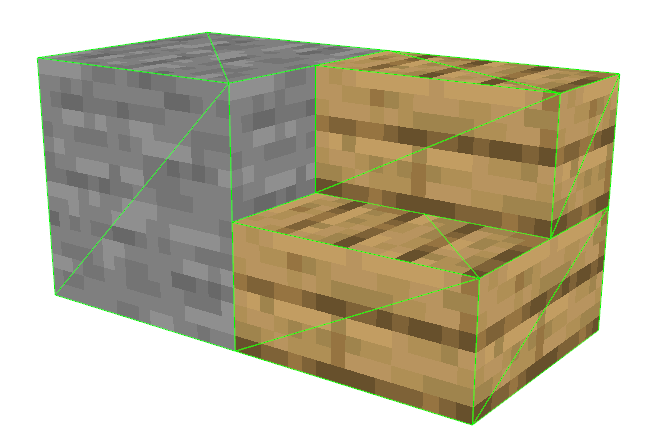
\includegraphics[width=0.8\textwidth]{../assets/culling/stair_next_to_stone.png}
		\end{center}
	\end{minipage}\hfill
\end{figure}
